\clearpage

\section{实验与结果分析}

基于第3节所描述的四个系统,我们学习了所有的四个工具\footnote{主要基于开源仓库\cite{figshareGreyboxFuzzing}开发},然后实现了这几个工具,并将其集成在一个统一的平台上。然后我们将这些工具在46个基准程序上进行测试,所涉及到的并发漏洞包括断言违规,死锁,内存读写错误等。

然后我们对四个系统进行实际的测试,运行了30个小时,得到最终的结果。获得数据后对结果进行处理,然后手动分析了各个工具在49个基准测试上挖掘出来的漏洞的真实性,这耗费了约20个小时。在此基础上,我们从几个系统性的维度对实验结果进行分析,这几个角度分别是:

\begin{enumerate}
\item 各个工具是否能够有效地发现漏洞。
\item 抽象调度空间对于工具有效性的贡献。
\item 工具在读取空间中探索的分布。
\item 其他利用读取关系的方式是否有效。
\end{enumerate}

通过对这些问题的分析,我们比较了各个工具的优劣,得到了它们具体的优势所在。通过对比分析各个系统的特性,我们系统地对各个技术以及其如何导致最终结果进行了完整深入地分析,并得到了一系列的结论。

然后我们将RFF应用到6个大型程序中,这些程序的代码行数是原本两个基准程序所有行数的14倍,平均每个程序增加7万行的测试代码。并使用SFuzz提升挖掘漏洞能力。

\subsection{实验配置}

\paragraph{基准}实验基于两个基准测试。分别是SCTBench\cite{githubGitHubMcimperialsctbench, wen2022controlled}和ConVul\cite{cai2019detecting}。选择这两个基准测试的原因是他们能够覆盖大多数的情况,包括漏洞的类型、软件的种类等。SCTBench结合了之前一些其他的基准测试,包括压缩工具\cite{yu2009case}、web引擎\cite{jalbert2011radbench}、并行数值计算等方面的软件。这些各种各样的软件,均利用了多线程的机制,其中不乏有超过几千行代码的软件,这些软件利用多线程的机制实现了复杂的操作,其中存在着并发漏洞。当工具对这些程序进行测试的时候,需要在复杂的代码逻辑中找到漏洞的位置,这对于工具的有效性提出了很高的要求,进而可以测试工具在挖掘并发漏洞方面的有效性。ConVul基准测试则包含了十个真实世界应用程序的并发漏洞。在此基础上我们还收集了6个真实世界的程序,如,平均每个程序的测试代码相比与SCTBench和ConVul增加7万行,以测试RFF在真实世界的大型应用中是否仍然可以迅速挖掘到并发漏洞。

\begin{table}
\caption{\label{tab:6app}应用程序信息}
\begin{spacing}{1.5}
\centering
\begin{tabular}{lllllll}
\toprule
 Programs & Description & Version & LOC \\
\midrule

xz & Data compression & 5.4.4 & 25K \\
pigz & Data compression & 2.4 & 6K \\
pxz & Data compression & 4.999.9beta & 410 \\
libvpx & Encode and decode videos & 1.41.1 & 310K \\
libwebp & Encode and decode images & 1.4.0 & 71K \\
x264 & Encode video streams & 0.164.r3107 & 56K \\

\bottomrule
\end{tabular}
\end{spacing}
\end{table}


\paragraph{对比工具}为了验证RFF和当前最先进的并发漏洞测试工具的能力,实验将RFF和PERIOD\cite{wen2022controlled},PCT\cite{burckhardt2010randomized} ,GenMC\cite{kokologiannakis2019model, kokologiannakis2021genmc}进行了比较。其中,PERIOD通过将多线程程序进行关键点切片,系统地对并发访问空间进行探索,同时利用linux的基于deadline的任务调度机制,实现了可控的多线程调度。PCT利用了随机的算法生成特定深度的调度来测试程序,保证了检测到并发漏洞的最小概率,我们这里实现了探索深度为3的PCT工具。我们还对RFF进行了切除实验,去除它的关键部分:抽象调度约束和reads-from反馈,我们基于POS算法实现了一个POS工具作为基准。除此以外,我们还实现了一个基于Q-Learning算法的工具,它同样利用到了reads-from relation,来证明RFF利用reads-from relation的方式时有效且成功的。还有一些其他的模糊测试工具例如MUZZ\cite{chen2020muzz}和CONZZER\cite{jiang2022context},由于无法得到源代码或进行实现,我们没有将其作为基准测试一起进行比较。

\paragraph{实验环境}本实验机器环境的CPU为Intel(R) Core(TM) i7-12700 2.10 GHz,软件环境为docker容器中的Ubuntu 20.04操作系统。每一个程序基准程序在将会对应的漏洞挖掘工具上运行5分钟。这个做法和之前的并发测试评估有所不同,这里使用超市而不是有限的调度次数,这样做的理由是,这样能够更加实际地比较每一种工具的开销,这包括工具插桩,调度序列化以及其他复杂的分析。每一个工具的测试都会运行20次得到平均值来考虑结果的方差。

\subsection{各个工具漏洞挖掘效率分析与对比}

\begin{figure}[ht]
    \centering
    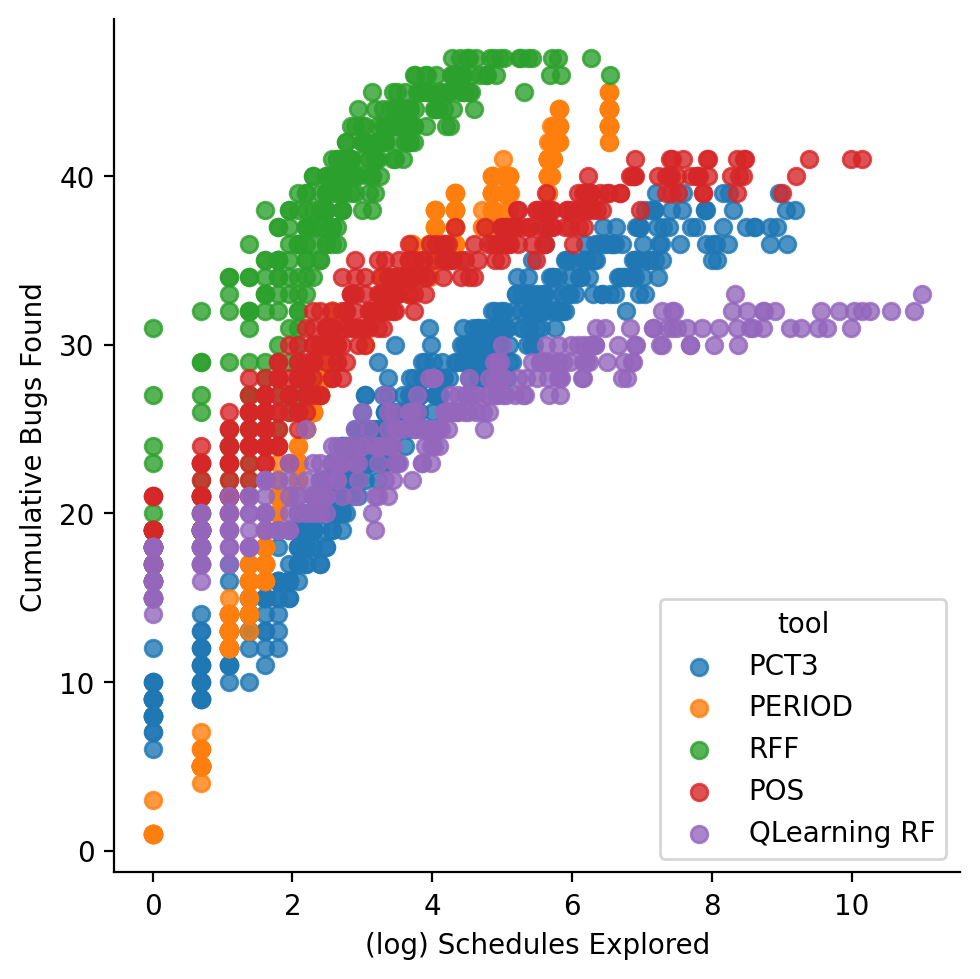
\includegraphics[width=.7\linewidth]{cum-scheds-to-bug}
    \caption{\label{fig:test1}随着测试的调度数增加发现的bug数量}
\end{figure}

我们将前面的几种工具应用在两个基准测试上运行,衡量的标准是每一个工具在特定schedule数量下发现的漏洞数量,结果在\autoref{tab:sample}中。在这几个工作中,GenMC无法在这些基准测试上运行,因此没有放在最终的比较中。PCT找到了39个程序的漏洞,PERIOD平均找到了45个程序的漏洞,而RFF平均找到了45个漏洞,这几乎是所有程序都成功检测到。在\autoref{fig:test1}中\footnote{本实验生成数据图片的脚本来自于\cite{wolff2024greybox}},我们展示了每一个工具经过一定的schedule之后,找到的漏洞的数量。这不仅反映了上面的结论,也就是RFF能比其他工具找到更多的漏洞,更反映了RFF能够在更少的schedule中找到更多的漏洞,这可以通过查看在每一个特定的schedule下,RFF几乎总是比其他的工具找到更多的漏洞。根据实验的数据,我们还可以得知,在33个程序中,RFF比PERIOD以更少的schedules找到漏洞,只有13个测试程序中,RFF比PERIOD以更多的schedules找到漏洞。对于两个同样是期望通过等价类来减少探索空间的工具来说,RFF利用的reads-from relation显然能够在找到等价类上有着更好的效果。

% \tabularxcolumn


\begin{table}
\begin{spacing}{1.5}
\caption{\label{tab:sample}平均找到第一个bug所需的调度数}
\zihao{7}
\begin{tabular}{lllllll}
\toprule
 & PCT3 & PERIOD & RFF & POS & QLearning RF \\
Benchmark &  &  &  &  &  &  \\
\midrule
CB/aget-bug2 & \textbf{ 1  $\pm$ 0  } & 9  $\pm$ 0  & \textbf{ 1  $\pm$ 0  } & \textbf{ 1  $\pm$ 0  } & \textbf{ 1  $\pm$ 0  } \\
CB/pbzip2-0.9.4 & \textbf{ - } & \textbf{ 45  $\pm$ 6 * } & \textbf{ 2  $\pm$ 0* } & \textbf{ - } & \textbf{ - } \\
CB/stringbuffer-jdk1.4 & 195  $\pm$ 174  & 27  $\pm$ 37  & \textbf{ 17  $\pm$ 18  } & \textbf{ 18  $\pm$ 23  } & 1405  $\pm$ 1592 \\
CS/account & 9  $\pm$ 7  & 10  $\pm$ 0  & \textbf{ 1  $\pm$ 0  } & \textbf{ 1  $\pm$ 0  } & 6  $\pm$ 8  \\
CS/bluetooth\_driver & 161  $\pm$ 162  & \textbf{ 9  $\pm$ 0  } & 64  $\pm$ 63  & 72  $\pm$ 79  & 155  $\pm$ 154 \\
CS/carter01 & 5  $\pm$ 4  & 4  $\pm$ 1 * & 2  $\pm$ 2  & 2  $\pm$ 1  & \textbf{ 1  $\pm$ 0  } \\
CS/circular\_buffer & 5  $\pm$ 4  & 3  $\pm$ 0  & \textbf{ 1  $\pm$ 1  } & \textbf{ 2  $\pm$ 1  } & \textbf{ 2  $\pm$ 1  } \\
CS/deadlock01 & 20  $\pm$ 20  & 3  $\pm$ 0  & 4  $\pm$ 3  & 4  $\pm$ 3  & \textbf{ 1  $\pm$ 0  } \\
CS/lazy01 & 10  $\pm$ 6  & 7  $\pm$ 2  & \textbf{ 6  $\pm$ 6  } & \textbf{ 5  $\pm$ 4  } & \textbf{ 12  $\pm$ 15  } \\
CS/queue & 12  $\pm$ 14  & 4  $\pm$ 1  & \textbf{ 1  $\pm$ 0  } & \textbf{ 1  $\pm$ 0  } & \textbf{ 1  $\pm$ 0  } \\
CS/reorder\_10 & 2356  $\pm$ 2302  & 27  $\pm$ 0  & \textbf{ 6  $\pm$ 4  } & \textbf{ - } & \textbf{ - }  \\
CS/reorder\_100 & \textbf{ - } & 297  $\pm$ 0  & \textbf{ 11  $\pm$ 9  } & \textbf{ - } & \textbf{ - } \\
CS/reorder\_20 & 2128  $\pm$ 2284  & 39  $\pm$ 0  & \textbf{ 6  $\pm$ 5  } & \textbf{ - } & \textbf{ - } \\
CS/reorder\_3 & 241  $\pm$ 336  & \textbf{ 6  $\pm$ 0  } & \textbf{ 7  $\pm$ 5  } & 223  $\pm$ 166  & 24700  $\pm$ 19638 *  \\
CS/reorder\_4 & 395  $\pm$ 320  & 9  $\pm$ 0  & \textbf{ 6  $\pm$ 4  } & 1464  $\pm$ 1829  & \textbf{ - }  \\
CS/reorder\_5 & 1126  $\pm$ 1045  & 12  $\pm$ 0  & \textbf{ 6  $\pm$ 4  } & 5942  $\pm$ 7210 * & \textbf{ - }  \\
CS/reorder\_50 & 4097  $\pm$ 5220 * & 129  $\pm$ 0  & \textbf{ 6  $\pm$ 4  } & \textbf{ - } & \textbf{ - }  \\
CS/stack & 2  $\pm$ 2  & 8  $\pm$ 0  & 2  $\pm$ 1  & 2  $\pm$ 2  & \textbf{ 1  $\pm$ 0  } \\
CS/token\_ring & 8  $\pm$ 6  & \textbf{ 2  $\pm$ 0  } & 5  $\pm$ 5  & 7  $\pm$ 5  & 12  $\pm$ 12   \\
CS/twostage & \textbf{ 9  $\pm$ 9  } & \textbf{ 4  $\pm$ 0  } & 12  $\pm$ 12  & 15  $\pm$ 16  & 336  $\pm$ 501   \\
CS/twostage\_100 & 848  $\pm$ 713 * & 690  $\pm$ 0  & \textbf{ 58  $\pm$ 57  } & \textbf{ - } & \textbf{ - }  \\
CS/twostage\_20 & 188  $\pm$ 168  & 76  $\pm$ 0  & \textbf{ 18  $\pm$ 14  } & 185  $\pm$ 215  & \textbf{ - }  \\
CS/twostage\_50 & 601  $\pm$ 440 * & 286  $\pm$ 0  & \textbf{ 32  $\pm$ 24  } & 1465  $\pm$ 979 * & \textbf{ - }  \\
CS/wronglock & 88  $\pm$ 98  & 4  $\pm$ 2  & \textbf{ 1  $\pm$ 0  } & \textbf{ 1  $\pm$ 0  } & 37  $\pm$ 32  \\
CS/wronglock\_3 & 40  $\pm$ 36  & 5  $\pm$ 1  & \textbf{ 1  $\pm$ 0  } & \textbf{ 1  $\pm$ 0  } & 37  $\pm$ 32   \\
Chess/InterlockedWorkStealQueue & 24  $\pm$ 19 * & 57  $\pm$ 0  & \textbf{ 1  $\pm$ 0  } & \textbf{ 1  $\pm$ 0  } & \textbf{ - }  \\
Chess/InterlockedWorkStealQueueWithState & 16  $\pm$ 0* & 224  $\pm$ 80  & \textbf{ 6  $\pm$ 4  } & \textbf{ 9  $\pm$ 9  } & 16  $\pm$ 14   \\
Chess/StateWorkStealQueue & 12  $\pm$ 0* & 249  $\pm$ 101  & \textbf{ 1  $\pm$ 0  } & \textbf{ 1  $\pm$ 0  } & \textbf{ - }  \\
Chess/WorkStealQueue & \textbf{ 12  $\pm$ 14  } & 57  $\pm$ 0  & \textbf{ 9  $\pm$ 7  } & \textbf{ 10  $\pm$ 9  } & \textbf{ - } \\
ConVul-CVE-Benchmarks/CVE-2009-3547 & 6  $\pm$ 5  & 2  $\pm$ 0  & \textbf{ 1  $\pm$ 0  } & \textbf{ 1  $\pm$ 0  } & \textbf{ 1  $\pm$ 0  } \\
ConVul-CVE-Benchmarks/CVE-2011-2183 & 9  $\pm$ 9  & 3  $\pm$ 0  & 2  $\pm$ 2  & 2  $\pm$ 1  & \textbf{ 1  $\pm$ 0  } \\
ConVul-CVE-Benchmarks/CVE-2013-1792 & 87  $\pm$ 65  & \textbf{ 13  $\pm$ 0  } & \textbf{ 19  $\pm$ 21  } & 50  $\pm$ 62  & 388  $\pm$ 361  \\
ConVul-CVE-Benchmarks/CVE-2015-7550 & 8  $\pm$ 7  & 3  $\pm$ 0  & 6  $\pm$ 5  & 7  $\pm$ 7  & \textbf{ 1  $\pm$ 0  } \\
ConVul-CVE-Benchmarks/CVE-2016-1972 & \textbf{ - } & \textbf{ 3  $\pm$ 0 * } & 36  $\pm$ 35  & 77  $\pm$ 66 * & 74  $\pm$ 39 *  \\
ConVul-CVE-Benchmarks/CVE-2016-1973 & 8  $\pm$ 5  & 6  $\pm$ 0  & \textbf{ 4  $\pm$ 3  } & 8  $\pm$ 10  & 5947  $\pm$ 6063   \\
ConVul-CVE-Benchmarks/CVE-2016-7911 & 16  $\pm$ 13  & 3  $\pm$ 0  & 14  $\pm$ 12  & 12  $\pm$ 11  & \textbf{ 1  $\pm$ 0  }  \\
ConVul-CVE-Benchmarks/CVE-2016-9806 & \textbf{ 5  $\pm$ 6  } & \textbf{ 6  $\pm$ 0  } & 14  $\pm$ 13  & 15  $\pm$ 10  & 664  $\pm$ 916   \\
ConVul-CVE-Benchmarks/CVE-2017-15265 & \textbf{ - } & \textbf{ 11  $\pm$ 0  } & 32  $\pm$ 37  & \textbf{ - } & \textbf{ - }  \\
ConVul-CVE-Benchmarks/CVE-2017-6346 & 15  $\pm$ 11  & 5  $\pm$ 0  & 4  $\pm$ 4  & 12  $\pm$ 12  & \textbf{ 1  $\pm$ 0  }  \\
Inspect\_benchmarks/boundedBuffer & 15  $\pm$ 16  & \textbf{ 8  $\pm$ 7 * } & \textbf{ 9  $\pm$ 8  } & \textbf{ 6  $\pm$ 5  } & 17  $\pm$ 15   \\
Inspect\_benchmarks/ctrace-test & \textbf{ 1  $\pm$ 0  } & 3  $\pm$ 0  & \textbf{ 1  $\pm$ 0  } & \textbf{ 1  $\pm$ 0  } & \textbf{ 1  $\pm$ 0  }  \\
Inspect\_benchmarks/qsort\_mt & 2515  $\pm$ 2838 * & \textbf{ 27  $\pm$ 0  } & 197  $\pm$ 171  & 646  $\pm$ 753  & \textbf{ - }  \\
SafeStack & \textbf{ - } & \textbf{ - } & \textbf{ - } & \textbf{ - } & \textbf{ - }  \\
Splash2/barnes & \textbf{ - } & \textbf{ 2  $\pm$ 0  } & 4  $\pm$ 3 * & \textbf{ 2  $\pm$ 2  } & \textbf{ 2  $\pm$ 1  }  \\
Splash2/fft & \textbf{ 1  $\pm$ 0  } & 2  $\pm$ 0  & \textbf{ 1  $\pm$ 0  } & \textbf{ 1  $\pm$ 0  } & \textbf{ 1  $\pm$ 0  } \\
Splash2/lu & \textbf{ - } & 2  $\pm$ 1  & \textbf{ 1  $\pm$ 0  } & \textbf{ 1  $\pm$ 0  } & 47  $\pm$ 38   \\
\bottomrule
\end{tabular}
\end{spacing}
\end{table}


\subsection{抽象调度有效性量化评估}

RFF中提出了一个新的抽象调度的概念,用来表示一个等价类,通过执行等价类中的一个具体调度,就能够测试这整个类,大大减少了探索的空间。而常规的POS中,并没有抽象调度这个概念,它是在实际的调度上进行操作的,这可能会导致其性能的不足。从\autoref{fig:test1}中的结果可以看到,在对SCTBench和ConVul这两个测试集的测试过程中,RFF能够在相同的schedule下发现更多的漏洞,并且随着schedule的增大,发现的漏洞数量的差距也在增大。RFF平均在每个程序上能够比POS多找到6个bug,这说明对于一些简单的容易触发的漏洞,POS也可以比较容易地挖掘,但是对于一些比较复杂的漏洞,POS即使在更多的schedule下也无法发现,而RFF可以稳定的发现更深层次的漏洞。

\subsection{调度空间探索效率量化分析}

\begin{figure}[ht]
    \centering
    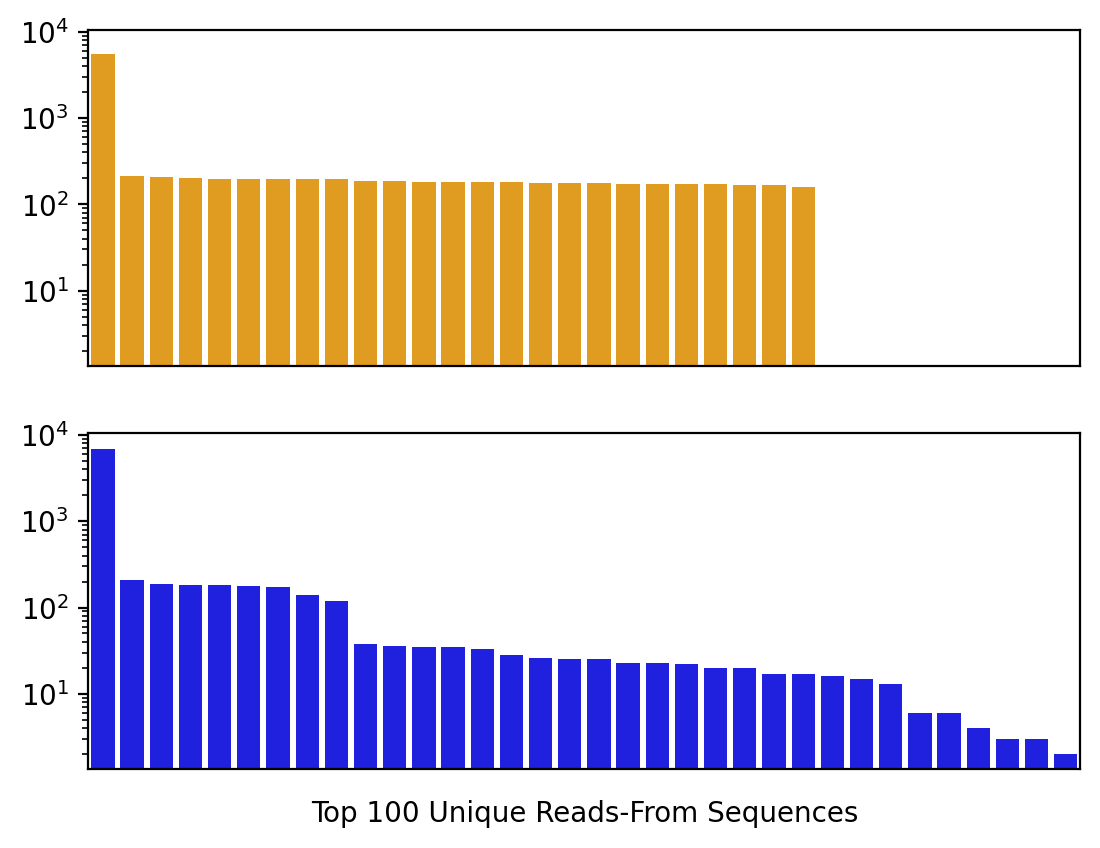
\includegraphics[width=.7\linewidth]{bar}
    \caption{\label{fig:test2}在SafeStack程序的10000次执行中,POS(上)和RFF(下)观察到的Reads-from relation频率}
\end{figure}

在对一个程序测试的过程中,如果一个调度可以有更多的reads-from relation,那么这个调度就更有可能触发程序的漏洞,因此模糊器如果能够被引导朝着更加有效的交错空间进行探索,那么就有可能发现更多的漏洞。我们测试了POS和RFF对同一个程序进行漏洞挖掘的过程中所用到的reads-from relation的数量,从\autoref{fig:test2}可以看到RFF能够检测到更多的reads-from relation,并利用这些reads-from relation产生有效的调度那行探索,相比之下,POS只能产生有限的reads-from relation。这是因为RFF在对当前的种子进行排序时,会更加倾向于那些拥有新的reads-from relation的种子,相比于POS的随机选取算法来说,这有助于模糊测试向着更有可能发现漏洞的交错空间进行探索。

\subsection{与Q-Learning技术的对比}
为了验证RFF基于模糊测试的方式的有效性,我们在这里还将它和另外一个同样利用了reads-from relation的框架进行对比。Q-Learning是一种强化学习技术,它可以从多个连续的状态中采取若干行动来获取最大化的奖励。为此,一个Q函数将每个状态行动映射到一个对应的分数$Q:S\times A \mapsto R$.这个分数,$Q(s_t, a_j)$,表示从状态$s_t$应该采取行动$a_j$的概率。再通过对这些概率进行抽样并确定下一个行动后,算法将会通过奖励函数更新对应状态行动的分数。这种方式可以用于并发测试,将每一个状态的调度决策视为一个行动。通过学习行动就能够学习到不同调度的优劣。

这里的目标是将Q-Learning作为一种替代的框架,利用reads-from relation,在并发程序中揭示错误,并探索新的控制流。具体来说,我们利用reads-from relation来区分Q-Learning中的不同状态,将具体调度$\sigma_{1\cdots t}$中的前t个事件的部分执行状态表示为到目前为止该执行中观察到的N个reads-from relation的累计哈希值

$$
h((e_{w_1}, e{r_1}), h((e_{w_2}, e{r_2}), \cdots, h((e_{w_N}, e{r_N}))))
$$

对于每一对$(e_{w_i}, e_{r_i})$,使$rf(e_{r_i})=e_{w_i}$。这里使用一个恒定的负奖励函数来处理观察到的状态行动对。从\autoref{fig:test1}中可以看出,Q-Learning RF在利用reads-from relation来挖掘两个数据集中的并发漏洞时并不像RFF那样有效。相对于RFF总共发现的45个程序的漏洞,它只发现了30个。RFF在30个程序的检测中能够以最少的调度数发现漏洞,而Q-Learning RF在15个程序中以最少的调度数发现漏洞。尽管少于RFF的30个,相比其他几个工具PERIOD、POS、PCT,Q-Learning RF能在更多的程序中以最少的调度数发现漏洞,这可能是由于在部分轨迹上的强化学习,导致Q-Learning不需要多次的测试就能成功挖掘已经学习过的漏洞模式。相比之下,RFF必须在完整的测试之后得到反馈,才能对下一步的测试进行调整。

\subsection{RFF在实际应用中的探索效率分析}

尽管RFF在SCTBench与ConVul这两个数据集上进行了测试,并取得了不错的效果。但是这两个测试集所测试的程序在复杂性上仍有所不足,而真实程序中的并发漏洞往往比较深,需要多条指令在一定的顺序下执行才能成功触发,同时这些指令之间的间隔可能比较远或是在不同的函数中,因此简单的样本测试程序并不足以完全反映这些并发漏洞挖掘工具的真实漏洞挖掘能力。

因此我们收集了多个真实世界中的应用程序,这些程序在复杂性上显著高于原本的样本测试程序,能够有效的检测工具的并发漏洞挖掘能力。
例如,在原本的测试集中,SCTBench总的代码行数仅为31000行,但是仅在我们收集的程序libvpx中就包含了31万行代码。在一个如此复杂的程序中,线程交错空间非常大,要穷举所有的交错种类并不可能,测试工具必须在探索效率和探索深度方面达到平衡才能有效地挖掘并发漏洞。

我们将RFF应用到pz、pxz、pigz、libvpx、libwebp、x264这六个应用程序中,尝试利用RFF挖掘这六个应用程序的漏洞,最终的结果如\autoref{fig:xz}、\autoref{fig:pxz}、\autoref{fig:pigz}、\autoref{fig:libvpx}、\autoref{fig:libwebp}、\autoref{fig:x264}所示:

\begin{figure}[ht]
    \centering
    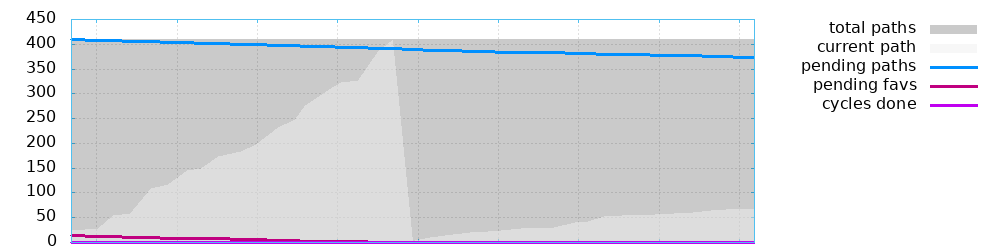
\includegraphics[width=0.8\linewidth]{xz}
    \caption{\label{fig:xz}xz}
\end{figure}

\begin{figure}[ht]
    \centering
    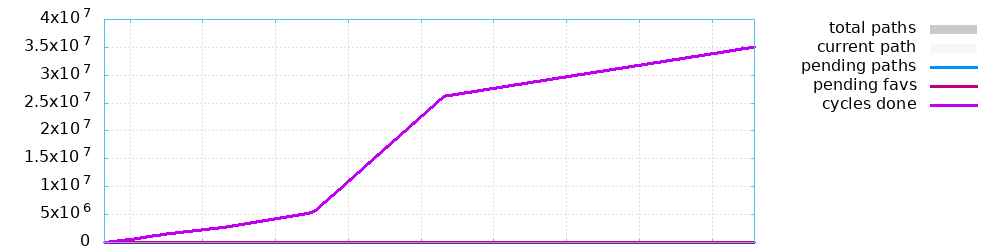
\includegraphics[width=0.8\linewidth]{pxz}
    \caption{\label{fig:pxz}pxz}
\end{figure}

\begin{figure}[ht]
    \centering
    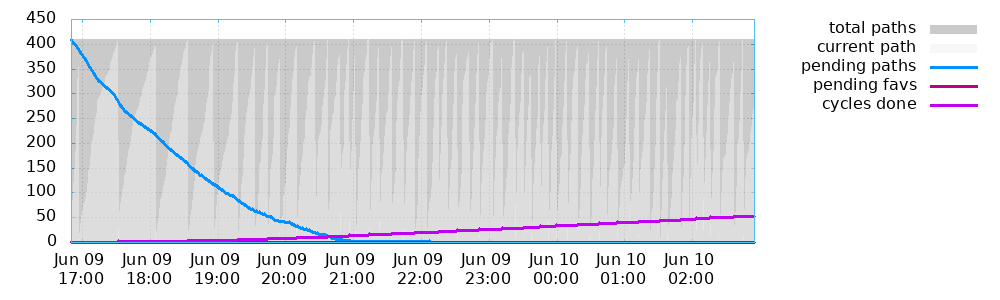
\includegraphics[width=0.8\linewidth]{pigz}
    \caption{\label{fig:pigz}pigz}
\end{figure}

\begin{figure}[ht]
    \centering
    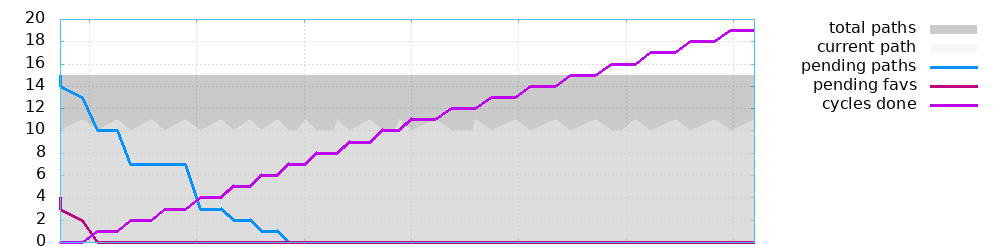
\includegraphics[width=0.8\linewidth]{libvpx}
    \caption{\label{fig:libvpx}libvpx}
\end{figure}

\begin{figure}[ht]
    \centering
    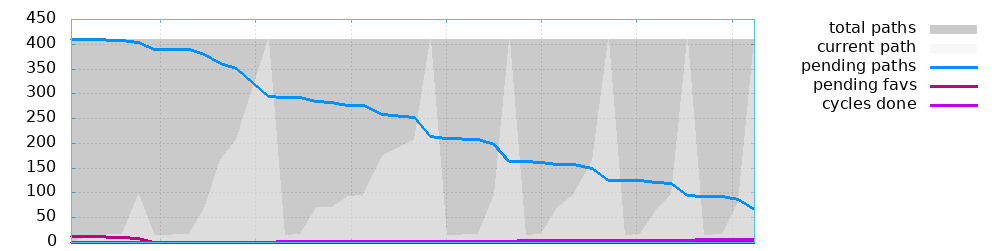
\includegraphics[width=0.8\linewidth]{libwebp}
    \caption{\label{fig:libwebp}libwebp}
\end{figure}

\begin{figure}[ht]
    \centering
    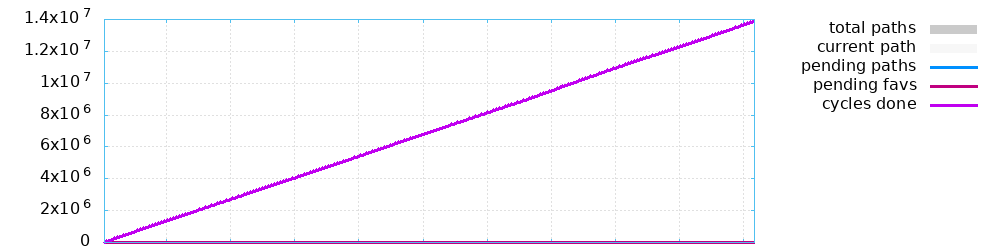
\includegraphics[width=0.8\linewidth]{x264}
    \caption{\label{fig:x264}x264}
\end{figure}

在这些测试中,随着测试时间的增加,RFF所探索的路径数量变化不同,在一些程序中可以迅速探索到多个路径,但是在具体路径的探索上可能并不深入,这说明可能在不同的路径中都存在着许多reads-from relation,这种情况下,RFF会对不同的路径进行均匀的探索。而在一些程序上,RFF会专注在一部分的路径上进行探索,这可能因为在这些路径上存在着大量的reads-from relations,进而影响的模糊测试的方向。

\subsection{初始种子对模糊测试的有效性影响评估}

我们在RFF的基础上提出了新的架构,这一架构通过为目标程序生成一个初始种子集合,提升RFF的漏洞挖掘效果。我们在pigz这一个程序上生成了相应的初始种子集合,并将这个测试用例和随机生成的初始种子同时在RFF上进行测试,如\autoref{fig:pigz-crash}、\autoref{fig:pigzmuzz-crash}所示,利用我们的工具生成的初始种子能够在相同时间内引导RFF挖掘到更多的并发漏洞。这也证明了3.5节中的分析,即常规程序输入同样能够影响并发漏洞的模糊测试效率,并且验证了SFuzz所生成的输入的确能够帮助模糊测试挖掘出更多的漏洞。

\begin{figure}[ht]
    \centering
    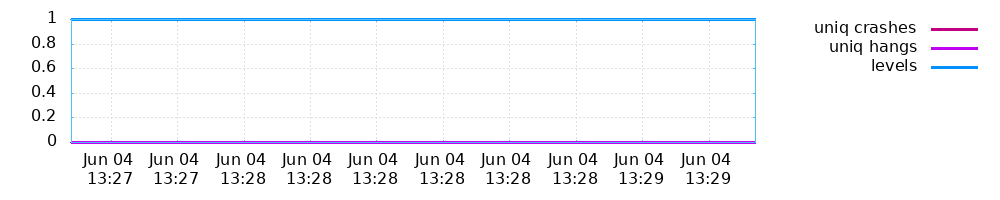
\includegraphics[width=0.8\linewidth]{pigz-crash}
    \caption{\label{fig:pigz-crash}Crashes found in pigz fuzzing}
\end{figure}

\begin{figure}[ht]
    \centering
    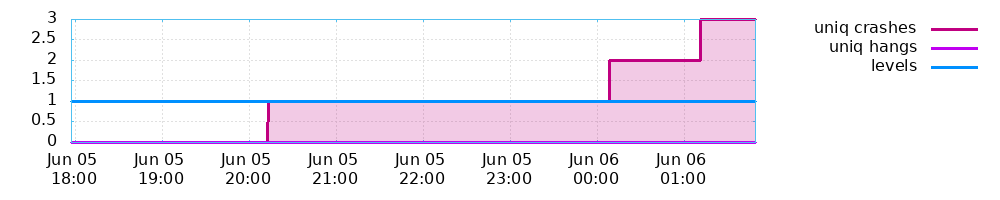
\includegraphics[width=0.8\linewidth]{pigzmuzz-crash}
    \caption{\label{fig:pigzmuzz-crash}Crashes found in pigz fuzzing with generated initial seeds}
\end{figure}

\clearpage

\section{总结与展望}

% \subsection{当前的相关工作}

% \subsubsection{针对并发漏洞的模糊测试器}

% 当前已经有多种针对不同对象的并发漏洞模糊测试器,例如用户程序\cite{chen2020muzz}、操作系统内核\cite{jeong2019razzer}、文件系统\cite{xu2020krace}以及网络协议\cite{pham2020aflnet}等。Razzer首先利用points-to分析,这是一种静态分析方法,能够找到不同访存指令之间的关系。基于得到的有关系的访存指令对,Razzer系统地对所有可能存在问题的指令对进行探索,但是这种方法由于引入了静态分析,会产生很多无用的指令对,降低了挖掘漏洞的效率。MUZZ\cite{chen2020muzz}在这个问题上注重引入低开销,通过引入覆盖率、线程上下文、schedule-intervention的反馈,对当前测试的输入进行评估,对种子集合进行筛选,减少需要探索的空间。KRace引入别名覆盖率来引导模糊测试器进行更好的模糊测试,别名覆盖率指的是一种关系的数量,这种关系里面,一条读取内存指令会读取另外一条写入指令的写入的值。通过这种方式,KRace对Linux内核的文件系统进行了模糊测试,利用别名覆盖率作为反馈指标,最终得到了比较好的结果。Conzzer\cite{jiang2022context}在函数级别的粒度上收集反馈信息,并基于这些信息来决定是否对相应的函数进行延迟操作。但是它只对两个线程上的两个函数进行分析,而不能扩展到三个线程及以上的情况。相比之下,RFF基于控制流和数据流只会在reads-from relation发生改变的时候产生改变这样一个事实,大大减少了模糊测试器需要测试的调度的数量,同时可以通过直接操作数据流的方式来改变调度。并且RFF在实际运行程序时的调度控制是细粒度化的,可以精确到指令级别,同时不会引入过大的开销。

% \subsubsection{随机并发测试}

% 有很多的工作尝试通过随机生成调度来挖掘漏洞,这相对于穷举测试来说,能够提升挖掘漏洞的效率,并且往往有概率上的保证。随机并发测试基于这样的事实,需要探索的调度空间是非常稀疏的,因此如果进行系统的探索,则有可能在一个没有错误的方向上进行大量的探索,这会严重影响工具的效率,甚至导致无法在有效的时间内检测出漏洞。一个比较有效的方式是,通过将不同的调度合并成同一个类,对每一个类中的一个例子进行探索,这样可以大大减少探索的数量。PCT\cite{burckhardt2010randomized}通过这种方式,将不同的交错进行分组,拥有相同的前缀行为的,会在同一个组下面进行测试。PPCT\cite{nagarakatte2012multicore}是PCT在多核情况的下延伸,在加快模糊测试的同时保证了探索的效率和准确度。RAPOS\cite{sen2007effective}提出了随机偏序采样算法,该算法部分消除了状态空间采样中的这种不均匀性,提高了测试的效率。基于RAPOS,POS\cite{yuan2018partial}通过对不同偏序的执行进行统一采样从而进一步提高了稳定发现bug的概率。并且目前基于随机的测试已经被扩展用于解决其他系统问题例如弱内存程序\cite{gao2023probabilistic, luo2021c11tester}和分布式系统\cite{ozkan2018randomized, ozkan2019trace, yuan2020effective}。

% \subsubsection{系统并发测试}

% 系统并发测试的优点是不会遗漏许多情形,但是缺点同样也很明显,就是在稀疏的交错空间里面的探索效率问题。Razzer就通过找到所有会访问相同地址的指令并对他们进行排序调度来达到测试的目的,但是即使仅仅考虑这些指令仍然需要搜索庞大的空间,同时静态分析会有很高的误报率。Maple\cite{yu2012maple}定义了一系列的可能会导致并发漏洞的内存访问模式,当遇到符合这些模式的指令时,就会对其进行测试。PERIOD\cite{wen2022controlled}将调度视作一系列的代码片段,每一个片段都是一个线程程序的一段,通过确定片段前缀,来不断探索更深层次的bug。

\subsection{未来研究展望}

当前在并发漏洞的挖掘上已经有了大量的探索,未来的探索方向主要有两个方面,分别是调度空间的缩减以及模糊测试流程的优化。

\subsubsection{交错空间的缩减}

并发漏洞难以发现的最大原因就是随着线程以及指令数量的增多,探索的空间将呈指数级别增长,目前的算力无法在合理的时间内对所有的情况进行探索。因此缩减探索空间是最直接,也应该是最有效的一种方式,但是目前针对交错空间的减少并没有一个特别好的效果,随机的方式在本质上并没有减少需要探索的空间,它仅仅是期望能够在空间中进行更有效的探索。本文中所提到的reads-from relation以及基于此构建的抽象事件以及抽象调度能够在一定程度上减少需要探索的情况。未来的工作可以通过理解并发漏洞的产生原因,对探索空间进行进一步的限制。

\subsubsection{模糊测试的优化}

当确定了需要探索的空间之后,就需要对不同的情况进行具体探索。前面提到的系统探索和随机探索都是可行的思路,但是两者都有着不可避免的缺陷,由于探索的空间过于稀疏,系统探索很难在探索的过程中找到有效的漏洞,特别是在初始的调度不合适的情况下,可能在大量尝试后仍然无法找到漏洞。随机探索对不同情况进行均匀的探索,可以有效缓解系统测试的问题。尽管随机探索能够保证以最低的概率检测到漏洞,但是这个概率仍然过小,无法高效率地检测到并发漏洞。

模糊测试通过筛选种子、变异、反馈等机制,将之前测试的结果进行分析得到更多信息,作为下一轮输入选取的指标,如果之前测试显示能够更加有效地对交错空间进行探索,那么就会继续在之前测试的用例上进行变异探索,如果没有很好的测试效果,就会改变方向。因此在模糊测试上可以从以下几个方面进行改进。首先选取一个更加合适的初始输入,因为模糊测试是一个连续的过程,它会将上一轮的输入进行变异,作为下一轮的输入。因此,一个好的初始输入,能够极大的提升模糊测试器发现并发漏洞的效率。其次,更好的变异算法。当我们对调度进行变异的时候,往往有众多的事件以及线程切换点,那么,如何从里面选取合适的变异点是比较关键的,这决定了探索能否高效的进行。最后还有引入新的反馈指标。更有效的反馈指标能够反映当前调度是否更有可能触发并发漏洞,因此也就能够更好地引导模糊测试器向着能够触发并发漏洞的调度前进。

\subsection{总结}

本篇文章研究了当前先进的并发漏洞检测工具,基于reads-from relation能够高效反映并发线程的数据流动关系的事实,构建了抽象调度来表示一个具体调度的集合,每个集合中的调度在数据流关系上都是等价的。在此基础上实现了对应的工具RFF以及PERIOD、PCT、POS多个先进工具并进行充分的实验,实验结果显示RFF能够以更少的时间在46个测试程序中发现45个程序的漏洞,比其他最好的工具平均少用73.4\%个调度检测出漏洞。实验结果还进一步证明SFuzz所生成的初始种子能够促使模糊测试挖掘到更多的并发漏洞。

% 而PCT和POS分别只能发现其中39个和38个程序的漏洞。PERIOD可以发现45个程序的漏洞,但是在其中39个程序上检测出漏洞所需要的调度数都比RFF更多,RFF所有程序平均比PERIOD少用73.4\%个调度检测出漏洞。这说明基于reads-from relation的RFF能够以更高的效率挖掘并发漏洞,并在多数情况下都能比其他的工具挖掘出更多的漏洞。